\part{Introduction}
\section{Motivation}
\begin{wrapfigure}{l}{0.3\textwidth}
    \centering
    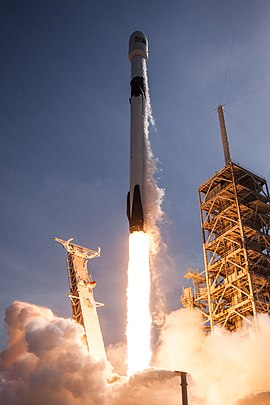
\includegraphics[width=0.3\textwidth]{falcon_9}
    \caption{Falcon 9}
    \label{fig:falcon_9}
\end{wrapfigure}
As we enter a new era of pushing the boundaries of space exploration back to the moon and beyond to Mars, so too must there be an effort to reevaluate our preparedness in developing and maintaining habitats which can support humans on these distant rocks. Much of the information about these enclosures has come from NASA research in the 70s and 80s, and independent projects like the Biosphere (early 1990s). The conclusion of all of these studies is that there is a lot to be understood when it comes to the complex system of recycling and regeneration which is required when resources, namely water and oxygen, are scarce and must be replenished from Earth. This project opens the door to further work in the area of simulation and modeling of these environments, tools which will be crucial in both feasibility and cost estimation studies in the coming decades.
\section{Background}
\subsection{Closed-Loop Systems}
\begin{wrapfigure}{r}{0.4\textwidth}
    \centering
    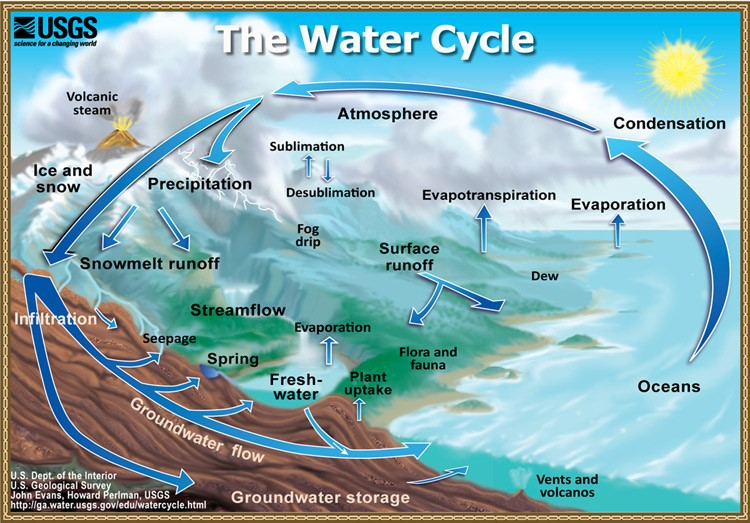
\includegraphics[width=0.4\textwidth]{water_cycle}
    \caption{The water cycle}
    \label{fig:water_cycle}
\end{wrapfigure}
A closed-loop system is a system in which all material components after initial closure are produced, consumed, and recycled within the system, such as the water cycle (Figure \ref{fig:water_cycle}). 

One of the earliest designs intended to replicate Earth’s natural regenerative systems (collectively called the biosphere) was Bios-3, a Russian experiment in regenerative feedback systems. At a cost of \$1 million in 1972, Bios-3 was the third generation in a series of increasingly complex demonstrations of materially closed-loop systems which used the natural processes of plants and algae to recycle carbon dioxide and provide nutrition for humans inside \cite{bios3}. 

The difficulty in designing such a system is that it requires understanding every environmental factor—biological, chemical, and ecological—through and through, and in a number of different configurations. Broadly, though, it is easy to envision what some of those components would be: O2, CO2, and trace gas levels and the associated chemical breakdown and respiration pathways, plant growth and interrelations with other communal species, human respiration and metabolism and requirements for food, water, and air quality, and the construction process for a fully-sealed environment. Ensuring that the crew operating the station are trained in all relevant processes, emergency procedures, and team dynamics is a part of the system which, though easy to ignore, should not be taken for granted. 
\subsection{NASA (1970s-Today)}
For researchers at NASA’s Ames Center, the summer of 1977 was an exciting time. A six-week long study was hosted covering a range of interests in Space Exploration and Human Settlements, which was at the time the “largest and most comprehensive investigation of space manufacturing and habitation,” covering topics in regenerative life-support systems, studies of efficient habitats in space, detection of asteroids for material collection, EM mass drivers for interorbital engines, and chemical processing of nonterrestrial material in space \cite{space_settlements}.

\begin{wrapfigure}{l}{0.3\textwidth}
    \centering
    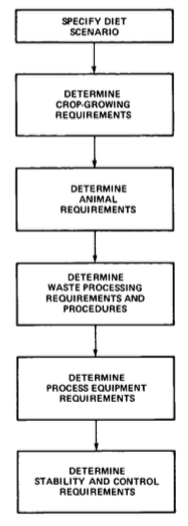
\includegraphics[width=0.3\textwidth]{CELSS_food}
    \caption{CELSS food system design}
    \label{fig:CELSS_food}
\end{wrapfigure}

In their review of regenerative life-support systems—of particular interest to the engineers a closed-loop habitat—they conclude that, in the long-term, a fully regenerative design should be implemented in order to maximize economic efficiency \cite{space_settlements}. Recognizing this, the researchers then outline a vision for investigating, evaluating and developing the technical components necessary for such systems. In their report, they discuss the limitations of the knowledge of the time including the nutritional requirements for humans not being fully understood; the lack of expertise as to how to rely on plants for reliable production of food, instead of consuming prepared foods; the uncertainty of containing and tracing environmental contaminants; the added complexity of integrating animals into the system; the handling of human waste and other organic scraps; and the risk of microbiological and other environmental hazards \cite{space_settlements}. For each of the systems, they outline initial ideas for research, as well as develop some specific frameworks around the systems such as the agricultural development model in Figure \ref{fig:CELSS_food}.

Throughout the 1980s and 90s, NASA made serious headway in investigating these phenomena with the Controlled Ecological Life Support System (CELSS) Program established as a result of the Ames study \cite{CELSS_1989,CELSS_1979}. The results of this decade-long program solidified groundwork for agricultural, human waste, and systems management investigations in the context of CLSS. One project, the Kennedy Space Center Breadboard project, set an original goal to “design, construct and test a ground-based CELSS at a one-person scale” \cite{breadboard}. This later evolved to “[evaluating] long-term operation of the biomass production system with increasing material closure” \cite{breadboard_waste}. By the end of the 1990s, there had been no actual experiment by NASA which studied humans in a fully closed-loop environment.

The work of the CELSS division would also be the last major program to look into closed systems, as funding slowly dwindled throughout the 90s. Though thanks to the construction of the ISS and the several manned space missions throughout the 2000s, there was a revamped effort to investigate the physiological effects of humans in space with the founding of the Human Research Program (HRP).

Founded in 2005, the HRP’s goal is to “provide human health and performance countermeasures, knowledge, technologies, and tools to enable safe, reliable, and productive human space exploration” \cite{HRP_intro} (Figure \ref{fig:hrp}). A number of “evidence reports” have been produced because of the program, which summarize and evaluate relevant bodies of research based on a critical 4-level metric of evidence credibility, ranging from Level I (“expert committee reports or opinions of respected authorities”) to Level IV (“at least one randomized, controlled trial”) \cite{HRP_intro}. They are independently verified yearly by the Institute of Medicine’s Committee on NASA's Research \cite{HRP_review}. 

\begin{wrapfigure}{r}{0.4\textwidth}
    \centering
    
\includegraphics[width=0.35\textwidth]{hrp}
    \caption{Human Research Program}
    \label{fig:hrp}
\end{wrapfigure}

One such evidence report, entitled “Risk of Inadequate Nutrition,” catalogs in great detail the broad range of micronutrients which support human health, and the experimental knowledge acquired from both ground-based and space missions \cite{HRP_nutrition}. This is a major success for closed-loop systems design, and the initial step in Spurlock and Modell’s agricultural design framework (Figure 3). Along with the work from the CELSS Program, it’s clear we have made some advancements in the Ames study objectives. Though there is still much to understand.

Most recently, NASA has been focusing on the social dynamics of sending teams into space, specifically under the notion that the researchers who sign themselves up to the journey will likely be making a one-way trip and thus be isolated from civilization once they arrive, confined to their small living space, a so-called “isolated, confined, and extreme (ICE)” environment. Even with all environmental, nutritional, and agricultural systems and control measures in place and understood among the community, there is still the potential that not everyone will remain content and that, as time progresses, there will be new and perhaps negative behavioral and psychological factors among team members.

\begin{wrapfigure}{l}{0.5\textwidth}
    \centering
    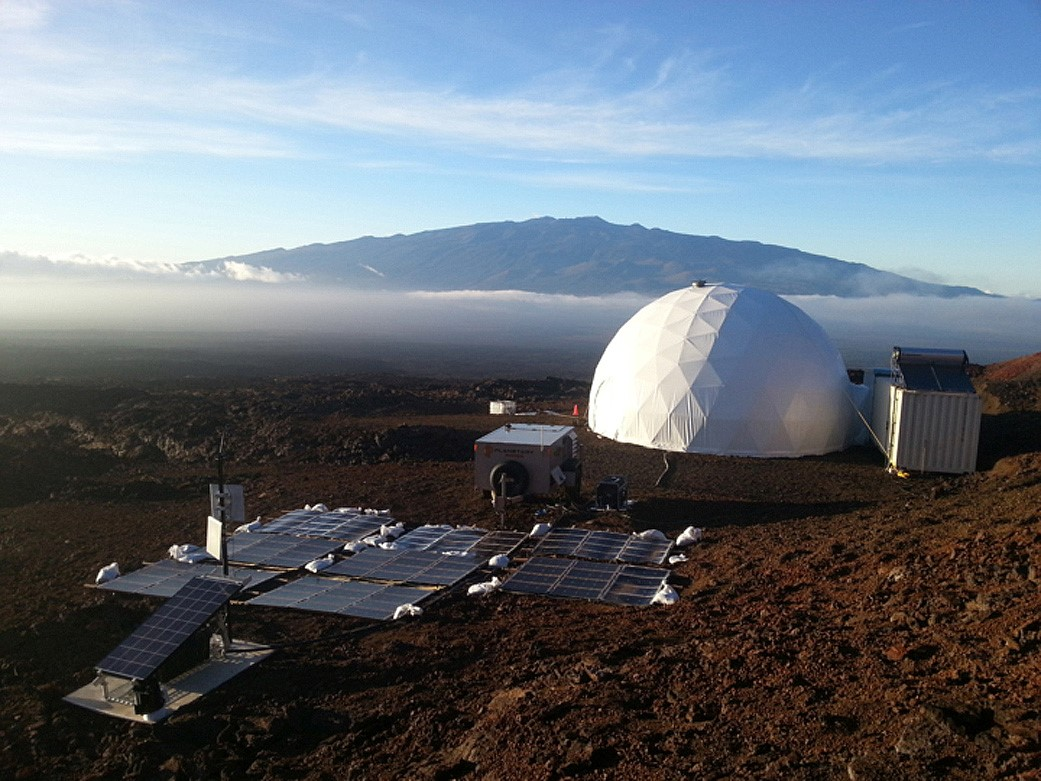
\includegraphics[width=0.5\textwidth]{HI_SEAS}
    \caption{NASA HI-SEAS}
    \label{fig:HI_SEAS}
\end{wrapfigure}

NASA’s ongoing missions at an isolated dome in the Hawaiian desert (Figure \ref{fig:HI_SEAS}), collectively named HI-SEAS, are providing some interesting data into the psychological and physiological effects of how to maintain cooperation and wellbeing in these ICE environments \cite{HI_SEAS}.  In their experiments, crew members are subjected to a simulated Mars environment, where they cannot leave their small enclosed habitat. One study by Dr. Peter Roma is investigating a novel system he calls COHESION, a computer game which systematically creates team-based tasks requiring interdependence and measures cooperation and other social factors \cite{social_dimensions}. Initial data suggests such a system can reduce stress, increase positive feelings, and facilitate achievement in teams \cite{HI_SEAS}. Another team led by Dr. Steve Kozlowski is hoping to gather critical data in regard to measuring physiological factors of long-term isolation as well as develop protocols for supporting teams in these environments. Both of theirs’s research will be published after the current round of HI-SEAS missions. And given the amount of uncertainty which remains in this relatively new field of study, this is surely a topic whose developments should be closely followed.

\subsection{Biosphere 2 (1980s-90s)}
\begin{wrapfigure}{r}{0.5\textwidth}
    \centering
    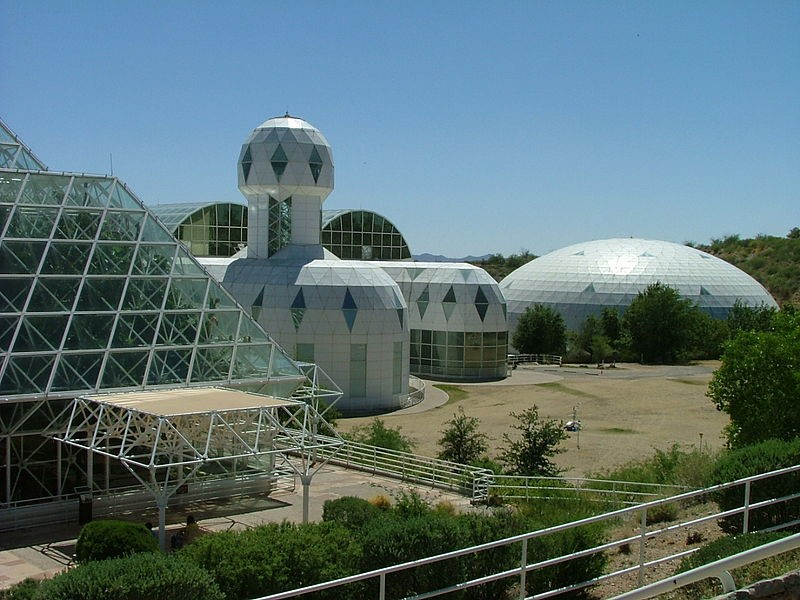
\includegraphics[width=0.5\textwidth]{biosphere_2}
    \caption{Biosphere 2}
    \label{fig:biosphere_2}
\end{wrapfigure}

In recognizing that Earth itself is a materially closed-loop and self-sustaining system, a team of researchers in the late-80s set out to design a scaled-down version of this biosphere, which they named affectionately Biosphere 2 (Figure \ref{fig:biosphere_2}). The goal was to replicate the different biomes of Earth under one enclosed structure, sealed from the outside world and able to support human life solely with the local constructed environment \cite{biosphere_intro}. This included growing food, providing a constant supply of freshwater, and controlling climatic variables and atmospheric gas concentrations. All the while, they were to record and measure levels of environmental variables and monitor the health of the researchers with on-site doctors \cite{dempster_conf}.

Biosphere 2’s design was unique for a number of reasons. Because of its level of complexity and fully enclosed nature (which had never been built on its scale before), there were a number of engineering challenges which needed to be tackled \cite{biosphere_intro}. One of the bigger challenges was due to the pressure differences which would arise with changing indoor humidity levels. In order to combat this, the engineers installed a system of two artificial lungs—large offsite chambers which could expand and deflate as needed. And then there was the matter of creating an airtight seal. To accomplish this, a number of high-grade stainless steel panels were welded together and used to line the concrete foundation. These, along with a 12mm silicone-caulked gap and sophisticated leak detection systems, helped to ensure an airtight seal for the entire structure \cite{biosphere_closed_loop}. In the end, the engineers achieved a leak rate of only 10\% per year \cite{biosphere_leakage}.

The majority of the research here came out of the two periods when researchers were sealed inside—the first, called Mission One, took place from 1991 to 1993 for a period of two years, and the second, Mission Two, was completed in 1994 for a period of 6 months \cite{biosphere_mission_one}. What came from this is an abundance of information in regard to material flows, or tracing the lifecycle of several of the organic and non-organic compounds in the system. After all, every atom which was there at the beginning was there in some form at the end (more or less)—the underlying beauty and necessity of studying in a closed-loop environment.

\begin{wrapfigure}{l}{0.5\textwidth}
    \centering
    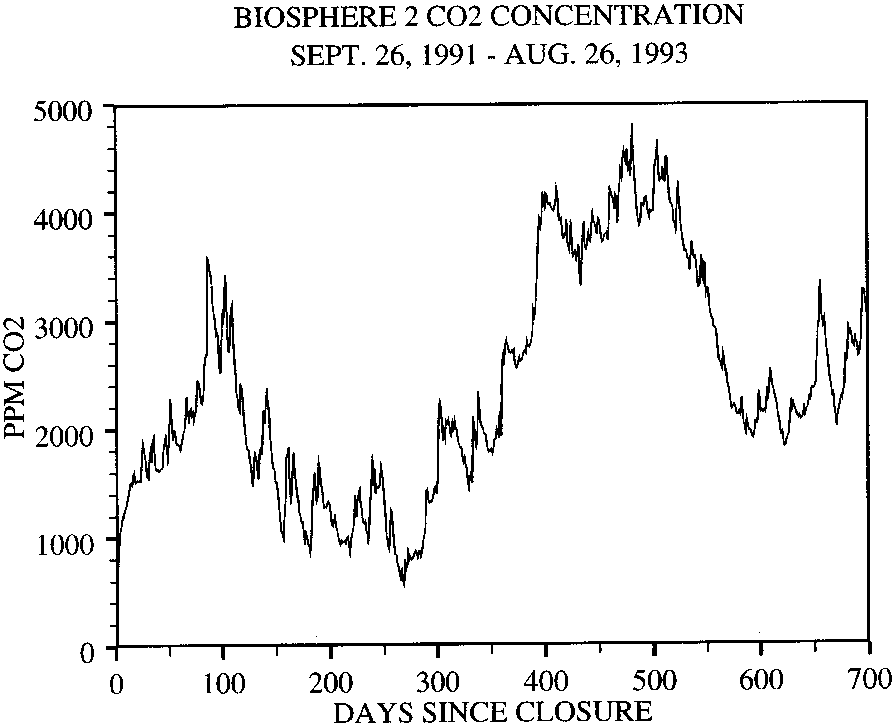
\includegraphics[width=0.5\textwidth]{biosphere_co2}
    \caption{Biosphere 2 CO$_2$ levels}
    \label{fig:biosphere_co2}
\end{wrapfigure}

Carbon dioxide was of particular concern and quickly rose in the first round of experiments as oxygen steadily declined (Figure \ref{fig:biosphere_co2}). The problem seemed to be that the concrete was absorbing a significant portion of atmospheric CO2, offsetting the balance between respiration of humans and plants, which should naturally be synchronized \cite{biosphere_design}.

Food was also a difficult system to control. And while the Biosphere’s creators designed the system to support a diet of 2500 kcal for each of the 8 crew members of Mission One, the average caloric intake in the first 6 months measured only $\sim$1780, rising to $\sim$2000 in the remaining time, leading to significant physiological changes including weight loss, decreased hormones, and decreased biochemical indicators such as cholesterol, blood sugar, and blood pressure. Dr. Roy Walford—who was a member of the Mission One crew and the supervising medical doctor—and his colleagues declared that despite all this, the crew members remained in “excellent” physical health \cite{biosphere_diet}.

The problem with the agriculture was that there were unexpectedly low light levels in the growing area due to the structural frame and double laminated glass which filtered away nearly 50\% of available sunlight \cite{biosphere_design}. The use of soils with high organic content led the soil to become highly saline over time and created extra problems with regards to plant biomass in the form of compost, which could not be easily reintegrated \cite{biosphere_agriculture}. And the decision to not use toxic pesticides ultimately caused further productivity decreases as crops suffered from increased pest damage and fungal disease \cite{biosphere_agriculture}.

Despite the many problems of Mission One, though, it did provide some positive insights as well. The fully functional constructed wetland which processed 240-290 gal/day of human effluent and supported 14 unique wetland species \cite{biosphere_wastewater}. Mission Two delivered expectedly better results with better agriculture yields and health and fewer issues overall due to a better understanding of the systems and learning from the mistakes of Mission One. In fact, the agricultural yields of Mission Two rose to higher than agrarian yields in Indonesia, Southern China, and Bangladesh, according to researchers \cite{biosphere_agriculture}.

Overall, although the design of Biosphere 2 would seem to be based in conflicting agendas of establishing regenerative life support systems and modeling the many biomes of Earth, the experiment ultimately resulted in a breadth of research and began preliminary testing of human coupling with their environment in CLSS---a claim which only Russia’s Bios-3 can match as of right now.